\chapter{Corrections and validation}\label{ch:audit}

Several recorded results were
corrected once the reference was matched, native work was priced, or the
evidence was replayed. Each correction is recorded in the source with a
dated note; frozen evidence is never rewritten. Figure~\ref{fig:audit}
shows the before and after values. Most corrections below moved
IC's position against rho \emph{down}, and several moved it from
apparently ahead of rho to behind it. Appendix~\ref{ch:corrections}
records two that moved it up: the byte-counter pricing rule and the
matched-rho re-measurement of the Joux--Vitse sieve.

\begin{figure}[t]
\centering
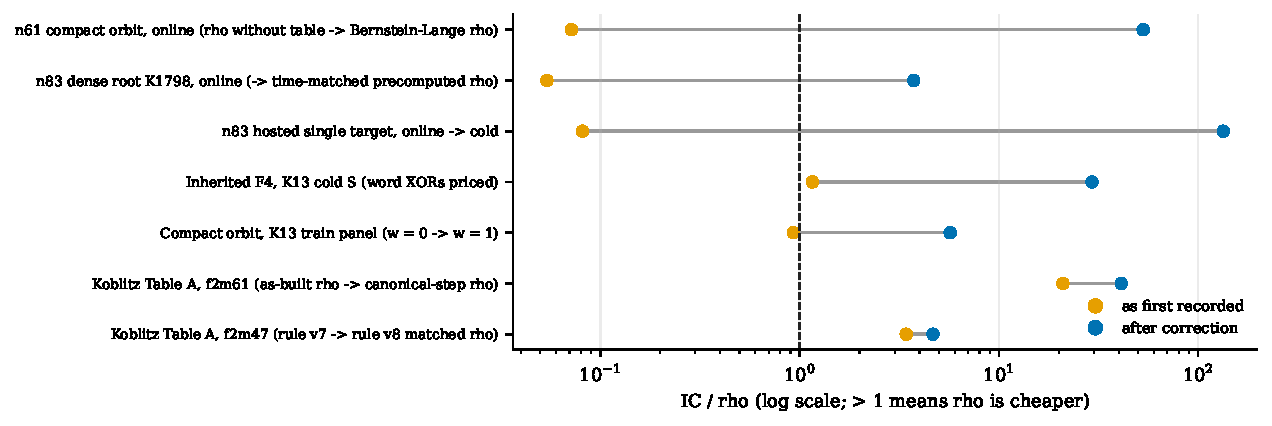
\includegraphics[width=\linewidth]{figures/fig-audit.pdf}
\caption[]{IC/rho as first recorded (orange) and after correction (blue), on
the boundary the correction used. Values left of the dashed line had
claimed IC ahead of rho. Sources: \art{figures/data-ledger.json}.}
\label{fig:audit}
\end{figure}

\section{Claims that did not survive}

\paragraph{1. Every online win is retired.} The one-target online ladder
compared IC \emph{with} a retained table against rho \emph{without} one
(Table~\ref{tab:audit-online}).

\begin{table}[t]
\centering\small
\begin{tabular}{@{}rlr@{}}
\toprule
$n$ & Reading & IC online over rho \\
\midrule
61 & strong rho, 64 targets & $13.94\times$ $[9.81,19.13]$ \\
83 & dense root index & $18.53\times$ \\
71 & hosted single target & $7.29\times$ \\
83 & hosted single target & $12.29\times$ \\
\bottomrule
\end{tabular}
\caption[]{The retired online wins: IC's online speed-up over rho with no
table, IC keeping its retained table.}
\label{tab:audit-online}
\end{table}
Given a distinguished-point table no larger than IC's pair table,
Bernstein--Lange preprocessing rho~\cite{bl2012} is $53$--$317\times$ faster
online at $n=41,53,61$ on the same 64 targets (benchmarks row
\texttt{20261014-ic-next10-09-equal-advice}). At $n=83$, rho with a table
matched to IC's set-up time or memory wins every pair: $3.74\times$
time-matched and $40.61\times$ memory-matched against K3300, and
$81.5$--$395.5\times$ against K600 (benchmarks row
\texttt{20261016-n83-precomputed-rho-control}). Cold, the hosted $n=83$
point is $133.7\times$ rho. Those online rows measured what a table buys,
and generic rho buys more per byte. The within-IC result survives: K1798's
probe reduction over K1500 at $n=83$ (from $300{,}021.9$ to $169{,}069.8$
probes per relation).

\paragraph{2. Pricing native work moved two arms.} Table~\ref{tab:audit-pricing}
gives both before and after.

\begin{table}[t]
\centering\small
\begin{tabular}{@{}lllr@{}}
\toprule
Arm & Reading & Rho & IC \\
\midrule
Inherited F4, $n=13$ & Boolean word XORs unpriced & $S=14.4$ & $S=16.7$ \\
 & priced & & $S=421.4$ \\
\addlinespace
Compact orbit, $n=13$ & earlier, lower bound & & $1.08\times$ rho \\
 & strong rho, $w=0$ & & $0.93$ \\
 & strong rho, $w=0.1$ & & $1.53$ \\
 & strong rho, $w=1$ & & $5.7\times$ \\
\bottomrule
\end{tabular}
\caption[]{The two arms moved by pricing native work. Inherited F4, whose unpriced $S$ was close to rho's:
\art{research/ecbench_rootfind_faster_20261014/}. Compact orbit at the
three band weights $w$; the pair is unresolved inside the band
(\art{research/ic_frontier_campaign_20261015/select/SELECTION.md}).}
\label{tab:audit-pricing}
\end{table}

The pricing change itself (\#1774, $0.002304$ GAE per word XOR) made every
earlier F4 $S$ a lower bound. A separate algorithmic change (\#1862) raised
counted work (\art{research/f4_pricing_jump_20261018/README.md}).

\paragraph{3. Matching the rho reference.} Table~\ref{tab:audit-rho} lists
the changes to the rho side.

\begin{table}[t]
\centering\small
\begin{tabular}{@{}lllr@{}}
\toprule
Change & Quantity & Scope & Factor \\
\midrule
Rule v8, matched rho & Koblitz gap raised & every size & $1.30$--$1.58\times$ \\
Standing rho improved & instruction count & \texttt{rho.signed\_frobenius\_strong} & $0.802\times$ \\
 & instructions per step & strong Koblitz rho & 718 instead of 1{,}196 \\
Better of $P\pm R$ & steps cut & prime side & $1.129\times$ \\
Signed $\sigma$ steps & GPU time cut to & ECC2K-130 & $0.961$--$0.970$ \\
\bottomrule
\end{tabular}
\caption[]{Changes to the rho reference and their factors. Rule v8:
Chapter~\ref{ch:distance}. The improved ecbench standing rho keeps
identical GAE, so counted-unit comparisons are unaffected; wall-time
comparisons against the older rho overstate IC by up to that factor. The
last two are rho studies, neither yet in a campaign arm.}
\label{tab:audit-rho}
\end{table}

\paragraph{3a. The matched reference re-priced every Table~B row.}
Through \S17 of the boundary ledger every prime and random-binary row was
divided by a frozen plain walk (16 jumps, two scalar multiplications per
walk start, distinguished points every $\sqrt r/8$). The matched
negation-map walk of 23 September replaced it, and the frozen walk was
replayed exactly on all 616 recorded runs of the ten re-priced reports
(\art{research/ic_rho_reference_20260923/README.md}).
Table~\ref{tab:fr-reprice} gives every row of the three round-5 reports.
\begin{itemize}
\item Ladder: best IC over rho $0.84$--$15.96$ before, $5.47$--$38.21$
  after. The one row below its rho, $0.84$ at 12 bits, reads $5.47$.
\item Headline: $4.19$ and $21.38$ before, $13.08$ and $45.29$ after.
\item Holdout: $4.74$--$16.79$ before, $12.67$--$37.07$ after.
\end{itemize}
The index-calculus $S$ is the same in both columns; only the reference
changed.

\begin{table}[t]
\centering\small
\setlength{\tabcolsep}{3.5pt}
\begin{tabular}{@{}llrrrrrr@{}}
\toprule
report & instance & $\log_2 r$ & $S_{\rm IC}$ & frozen $S_\rho$ & matched $S_\rho$ & IC/frozen & IC/matched \\
\midrule
ladder & \texttt{bench-10bit} & 9.68 & 22.85 & 22.66 & 3.605 & 1.01 & 6.34 \\
ladder & \texttt{bench-12bit} & 11.93 & 15.62 & 18.58 & 2.855 & 0.84 & 5.47 \\
ladder & \texttt{bench-14bit} & 13.99 & 13.07 & 8.91 & 2.034 & 1.47 & 6.43 \\
ladder & \texttt{bench-16bit} & 15.99 & 11.68 & 6.36 & 1.740 & 1.84 & 6.71 \\
ladder & \texttt{bench-18bit} & 18.00 & 8.41 & 4.20 & 1.446 & 2.00 & 5.82 \\
ladder & \texttt{bench-20bit} & 20.00 & 10.72 & 2.68 & 1.292 & 3.99 & 8.30 \\
ladder & \texttt{generated-22bit-3290411} & 21.65 & 12.77 & 2.98 & 1.216 & 4.28 & 10.50 \\
ladder & \texttt{generated-24bit-10935329} & 23.38 & 13.97 & 3.93 & 1.038 & 3.55 & 13.46 \\
ladder & \texttt{random-binary-n15-b524b} & 13.99 & 26.31 & 8.36 & 2.013 & 3.15 & 13.07 \\
ladder & \texttt{random-binary-n18-b6507} & 15.00 & 21.30 & 7.56 & 2.006 & 2.82 & 10.62 \\
ladder & \texttt{random-binary-n21-b1b6f3b} & 20.00 & 24.39 & 3.18 & 1.356 & 7.66 & 17.99 \\
ladder & \texttt{random-binary-n24-b5fc9da} & 21.00 & 27.24 & 2.52 & 1.183 & 10.83 & 23.03 \\
ladder & \texttt{random-binary-n27-b845462} & 24.41 & 36.93 & 2.31 & 0.966 & 15.96 & 38.21 \\
\addlinespace
headline & \texttt{generated-24bit-10935329} & 23.38 & 13.73 & 3.28 & 1.049 & 4.19 & 13.08 \\
headline & \texttt{random-binary-n27-b845462} & 24.41 & 46.52 & 2.18 & 1.027 & 21.38 & 45.29 \\
\addlinespace
holdout & \texttt{generated-22bit-2987209} & 21.51 & 14.20 & 2.96 & 1.121 & 4.80 & 12.67 \\
holdout & \texttt{generated-24bit-12832957} & 23.61 & 12.62 & 2.66 & 0.878 & 4.74 & 14.38 \\
holdout & \texttt{random-binary-n24-bf19f6f} & 21.00 & 28.73 & 2.43 & 0.963 & 11.81 & 29.84 \\
holdout & \texttt{random-binary-n27-b7ade7fe} & 26.00 & 33.46 & 1.99 & 0.903 & 16.79 & 37.07 \\
\bottomrule
\end{tabular}

\caption[]{Round-5 boundary reports re-priced against the matched rho. $S$
in GAE per $\sqrt r$; $S_{\rm IC}$: best of nine recipes; frozen $S_\rho$:
the plain walk used through \S17; matched $S_\rho$: the negation-map walk.
The ladder rows are leaderboard Table~B
(Table~\ref{tab:fr-boardB}). Source:
\art{research/ic_rho_reference_20260923/analysis.json}
(\texttt{tables.boundary}). Data: \art{figures/data-fr-leaderboard.json}.}
\label{tab:fr-reprice}
\end{table}

\paragraph{4. A replay regression, and its root cause.} The root-finder
ecbench session was recorded with a replay certificate of 120 of 168
identical records; the 48 mismatches were all in inherited F4's word-XOR
counts. On \texttt{main} of 19 October it replayed only 72 of 168, with
mismatches in all four index-calculus arms.
\begin{itemize}
\item \emph{First diagnosis} (20 October). A cross-ISA replay found that
  with the x86-only BMI2 branch disabled, x86 reproduces all 168 of 168
  records, and so does an aarch64 build under emulation
  (\art{research/validation_sweep_20261019/D-known-issues/item1_cross_isa_20261020/RESULT.md}).
\item \emph{Cause, stated precisely} (26 October addendum). At the recorded
  commit, BMI2 availability decided whether F4's row specialisation was
  \emph{eager} (every kept row rewritten at once and charged per row) or
  \emph{lazy} (rewritten on first read). The two differ in the quantity
  charged, for example $301{,}961$ against $300{,}531$ word XORs. Since
  \#2043 every host is eager and the two eager paths charge identical
  counts. Sessions now record the version of the F4 accounting they were
  made under
  (\art{research/validation_sweep_20261019/D-known-issues/ADDENDUM-20261026-item1-accounting.md}).
\end{itemize}
Archived sessions recorded with the lazy charge cannot replay on
\texttt{main}. That is a change of definition, not a dependence on the host.
Scalars, trial counts and charged group operations are unaffected.

\paragraph{5. Reported cells that compared unlike statistics.} The
u64-rootbatch rank and per-target cells compared a fastest run with a
median, and were corrected from $2.95\times$ and $6.09\times$ to $2.47\times$
and $5.00\times$ (Chapter~\ref{sec:koblitz}). The $n=83$ stacked producer's
``$360\to94.4$'' cold-gap history mixed a ratio from another run; paired
within the run it is $305.8\to94.4$ (Chapter~\ref{sec:koblitz}).

\paragraph{6. Results resting on faulty code or wrong references.}
\begin{itemize}
\item \emph{Plane-quartic IC.} Its $S$ values of $650{,}896$ to
  $3.79\cdot10^7$ rest on a degree-3 reduction in
  \art{research/ghs_cubic_quartic_ic_20261012/quartic_ic.rs} that merges
  distinct classes (reported in an open pull request). Recoveries are still
  checked against the planted scalar, but relation counts and $S$ are
  unverified. Canonical $\mathrm{Pic}^0$ keys later fixed the merge
  (\art{research/quartic_pic_canonical_20261018/}). The N4 and N4~v2
  measurements of Chapter~\ref{ch:distance} use the fixed code; the
  withdrawn values are the earlier toys only.
\item \emph{Volcano census crater.} A claim that IC is 22--25\% cheaper on
  the volcano crater was withdrawn, because the crater's rho reference
  should have been the cubic-automorphism rho. Against it, IC is
  $84.9\times$ rho at $w=0$
  (\art{research/volcano_ecdlp_census_20261017/REPORT.md}, erratum A3).
\end{itemize}

\paragraph{Reading.} None of these corrections removes an IC improvement
against its own incumbent. They correct the \emph{distance to rho}, which
is the quantity most exposed to an unmatched reference or an unpriced
counter. This is why the gate of \S\ref{sec:gate} asks for a matched,
band-priced rho on every row.

\section{Validation status}\label{sec:gate}

Since 19 October no row may enter the index-calculus leaderboard or
\art{benchmarks/README.md} without three pieces of evidence, named by the
evidence directory's \texttt{VALIDATION.json}
(\art{docs/VALIDATION_GATE.md}):
\begin{itemize}
\item an independent replay certificate with verified scalars;
\item an independent validator report that recomputes every headline
  number;
\item a matched rho reference: the strongest available, in the same unit
  and the same binary, priced across the §5a band.
\end{itemize}
On 29 October, \textbf{19 of the 28 leaderboard rows are validated}
(\art{docs/ic/leaderboard.json}, \texttt{validation\_gate.status\_counts}).

Table~\ref{tab:audit-validation} gives the status by leaderboard table.

\begin{table}[t]
\centering\small
\begin{tabular}{@{}l>{\raggedright\arraybackslash}p{0.2\linewidth}r>{\raggedright\arraybackslash}p{0.16\linewidth}lr@{}}
\toprule
Table & Scope & Rows & Status & Rho reference & IC/rho \\
\midrule
B & prime and random binary, one target & 13 & validated 24 October & matched negation-map & $5.47$--$38.21\times$ \\
 & & & & across the band & $4.05$--$54.76\times$ \\
\addlinespace
A & Koblitz descent, one target & 6 & validated at baseline v7 & as-built, same process & $3.43$--$11.5\times$ \\
 & & & & matched, rule v8 & $4.67$--$18.07\times$ \\
\addlinespace
C & 32-target batch & 9 & pre-gate & none matched, no band & \\
\addlinespace
--- & components outside A--C & (2) & validated & & \\
\bottomrule
\end{tabular}
\caption[]{Validation status of the leaderboard on 29 October. Table~B
validated on 24 October (\art{research/ic_validation_gate_20261024/}):
1{,}257 runs replay identically in a fresh process; 1{,}578 of 1{,}578
negative controls are rejected by an independent verifier; 52 headline
numbers recompute to relative $10^{-9}$; index calculus stays above rho at
every band weight. Table~A (64 targets per size) validated at baseline v7
(\art{research/ic_tool_program/rule/v7/}); the sweep flags the reference as
only partly adequate, and the rule~v8 row is from
Chapter~\ref{ch:distance} (rule v8 also carries a \texttt{VALIDATION.json},
\art{research/ic_tool_program/rule/v8/VALIDATION.json}; the board has not
been regenerated on it). Table~C's replays and recomputations pass, but
no matched rho with a band exists for them. The component row is not
counted in the 28 rows; it names two of several validated components
(\art{docs/ic/leaderboard.json} has more, among them the generator-orbit
and aimed-gather components): the prime-field base-size tuning and the post-Gröbner linear stage
(\art{research/prime_base_oracle_tuning_20261029/VALIDATION.json},
\art{research/postgb_linear_stage_20261026/validation/VALIDATION.json}).}
\label{tab:audit-validation}
\end{table}
Validation says the numbers are what the archive says, and that the
reference is fair. \textbf{No validated leaderboard row is below its
reference.} The one validated measurement below a matched rho is the
Joux--Vitse sieve route on the \texttt{jv\_cover} weak class
($0.0065\times$, $p=1511$, \texttt{VAL-20261103-c31c76};
\S\ref{sec:jac-jv}). It is not a leaderboard row, never has prime order,
and has no pcc claim. The 19 validated board rows each have a pcc
measurement claim, of standing unverified.

\paragraph{The benchmarks table.} \art{benchmarks/README.md} on
\texttt{origin/main} (\texttt{05f7382689}) admits 145 rows
(Table~\ref{tab:fr-benchcount}). Twenty link a \texttt{VALIDATION.json} in
the row; 112 are listed in \art{benchmarks/PRE_GATE.json} and render as
unvalidated (pre-gate); 13 do neither. Fifteen of the twenty measure an
index-calculus pipeline or one of its stages, and Table~\ref{tab:fr-bench}
gives the distance to rho each of them states. Thirteen state IC above rho in
every cell and at every weight they report. The genus-3 linear-algebra row is below rho at
$w=0$ ($0.38\times$) and above it at $w=0.1$ and~1, so unresolved across
the band. The Joux--Vitse Hilbert-stop row states only a slope of $S$ over
rho ($-2.27$) and a lower bound on IC.

\begin{table}[t]
\centering\small
\begin{tabular}{@{}lrrrr@{}}
\toprule
row date & \texttt{VALIDATION.json} linked & unvalidated (pre-gate) & neither & all \\
\midrule
2026-10 & 18 & 112 & 13 & 143 \\
2026-11 & 2 & 0 & 0 & 2 \\
\midrule
all & 20 & 112 & 13 & 145 \\
\bottomrule
\end{tabular}

\caption[]{Rows of the admitted benchmarks table by date and gate
standing. ``Linked'': the row links its \texttt{VALIDATION.json};
pre-gate: the row's slug is in \art{benchmarks/PRE_GATE.json}; neither:
admitted under the 24 October gate audit without a file linked in the row.
Counted by \art{figures/make_tab_fr.py}. Data:
\art{figures/data-fr-bench.json}.}
\label{tab:fr-benchcount}
\end{table}

\begin{table}[t]
\centering\scriptsize
\begin{tabularx}{\linewidth}{@{}l>{\raggedright}p{4.2cm}>{\raggedright\arraybackslash}X@{}}
\toprule
date & entry and what it measures & distance to rho, as the row states it \\
\midrule
11-02 & \art{20261102-e39-pivot-rules}: $k=4$ GLS/$V_4$ chain solve, pivot rules (E39) & rho ahead everywhere, closest row F $5.18\cdot10^{3}$$\times$ (0 GAE) and $1.11\cdot10^{5}$$\times$ (1 GAE) rho \\
11-02 & \art{20261102-e40-macaulay-entries}: same, Macaulay build stores rows from the lead column (E40) & rho ahead everywhere, closest row $6.00\cdot10^{3}$$\times$ / $1.58\cdot10^{4}$$\times$ / $6.17\cdot10^{4}$$\times$ \\
10-31 & \art{20261031-e32-handover-ladder}: same, handover ladder $p=101$--$3089$, 33 curves (E32) & rho ahead on all 33 curves at every weight; median distance $2.07\cdot10^{4}$$\times$ (p = 101) to $1.54\cdot10^{3}$$\times$ (p = 3089) at 0 GAE; best curve 1,143$\times$ \\
10-30 & \art{20261030-e27-walk-karatsuba}: matched walk with Karatsuba products (E27) & distance remaining $6.39\cdot10^{3}$--$4.06\cdot10^{5}$$\times$ at 0 GAE, rho ahead across the \S5a band \\
10-24 & \art{20261024-e31-chain-solve}: chain solve, solvers A and B (E31) & best S/rho $4.42\cdot10^{3}$ (A) at 0 GAE, rho ahead at every weight \\
10-29 & \art{20261029-jv-cover-hilbert-stop}: Joux--Vitse cover, F4 Hilbert stop & log--log slope of S/rho $-$2.27; IC is a lower bound \\
10-29 & \art{20261029-ic-aimed-gather}: Koblitz $n=53$ aimed gather, collect phase & the board's rule v7 row (IC 8.146 vs rho 1.159 S, 7.03$\times$) predates the change \\
10-29 & \art{20261029-ic-packed-filter}: prime pair-table packed filter, 32 bits & dgbf / rho-neg 31.47 / 31.50 / 31.63 \\
10-29 & \art{20261029-prime-fb-size-20bit}: prime base size $N=32\to45$, 20 bits & distance to rho 9.47 $\to$ 7.75 (w = 0), 12.88 $\to$ 9.35 (w = 1) \\
10-28 & \art{20261028-d4-char2-frob-roots}: $k=4$ characteristic two, Frobenius roots & IC/rho at m = 14: 4.27 $\to$ 3.48 (w = 0), 2.13 $\to$ 1.74 (w = 1) \\
10-27 & \art{20261027-postgb-linear-stage}: post-Gröbner linear stage, \texttt{jv\_cover} & S over the negation-map rho 257--1310 (pooled 497 at w = 0, 64 at w = 1) \\
10-17 & \art{20261017-isogeny-volcano-cost-v2}: IC yield across volcano levels & IC/rho 17--170$\times$ at w = 0 \\
10-18 & \art{20261018-blindspots-fp2-gaudry-k2}: Gaudry $k=2$ over $\FF_{p^2}$, 24--40 bits & best arms ic-b and ic-c2 50x and 52x rho at 40 bits (w=0), 22x and 14x (w=1) \\
10-18 & \art{20261018-blindspots-prime-m4-cells}: prime arity $m=4$, 16--28 bits & 6.5x to 35.6x across w = 0, 0.1, 1 \\
10-18 & \art{20261018-blindspots-genus3-la-exponent}: genus-3 linear algebra, $b=20$ & below rho at w=0 (0.38x) and above it at w=0.1 (1.6x to 2.6x) and w=1 (3.7x to 6.5x) \\
\bottomrule
\end{tabularx}

\caption[]{The 15 admitted benchmark rows with a linked
\texttt{VALIDATION.json} that measure an index-calculus pipeline or stage,
with the distance to rho as each row's headline states it (excerpts; every
number checked against the row by \art{figures/make_tab_fr.py}). The other
five linked rows are a strong-rho engineering round and four studies of
generic walks and pencil models priced against rho. Several rows state
their validation ``with caveats'' (same-host replay, one session). Source: \art{benchmarks/README.md}. Data:
\art{figures/data-fr-bench.json}.}
\label{tab:fr-bench}
\end{table}

The theory of Part~\ref{part:theory} has a different standard of evidence:
\begin{itemize}
\item written proofs, which still need expert review;
\item independently checked certificates;
\item Lean for the finite and algebraic identities only.
\end{itemize}
Each theorem there names its tier.
